\documentclass[
  shownotes,
  xcolor={svgnames},
  hyperref={colorlinks,citecolor=DarkBlue,linkcolor=DarkRed,urlcolor=DarkBlue}
  , aspectratio=169]{beamer}
\usepackage{animate}
\usepackage{amsmath}
\usepackage{amsfonts}
\usepackage{amssymb}
\usepackage{pifont}
\usepackage{mathpazo}
%\usepackage{xcolor}
\usepackage{multimedia}
\usepackage{fancybox}
\usepackage[para]{threeparttable}
\usepackage{multirow}
\setcounter{MaxMatrixCols}{30}
\usepackage{subcaption}
\usepackage{graphicx}
\usepackage{lscape}
\usepackage[compatibility=false,font=small]{caption}
\usepackage{booktabs}
\usepackage{ragged2e}
\usepackage{chronosys}
\usepackage{appendixnumberbeamer}
\usepackage{animate}
\setbeamertemplate{caption}[numbered]
\usepackage{color}
%\usepackage{times}
\usepackage{tikz}
\usepackage{comment} %to comment
%% BibTeX settings
\usepackage{natbib}
\bibliographystyle{apalike}
\bibpunct{(}{)}{,}{a}{,}{,}
\setbeamertemplate{bibliography item}{[\theenumiv]}

% Defines columns for bespoke tables
\usepackage{array}
\newcolumntype{L}[1]{>{\raggedright\let\newline\\\arraybackslash\hspace{0pt}}m{#1}}
\newcolumntype{C}[1]{>{\centering\let\newline\\\arraybackslash\hspace{0pt}}m{#1}}
\newcolumntype{R}[1]{>{\raggedleft\let\newline\\\arraybackslash\hspace{0pt}}m{#1}}


\usepackage{xfrac}


\usepackage{multicol}
\setlength{\columnsep}{0.5cm}

% Theme and colors
\usetheme{Boadilla}

% I use steel blue and a custom color palette. This defines it.
\definecolor{andesred}{HTML}{af2433}

% Other options
\providecommand{\U}[1]{\protect\rule{.1in}{.1in}}
\usefonttheme{serif}
\setbeamertemplate{itemize items}[default]
\setbeamertemplate{enumerate items}[square]
\setbeamertemplate{section in toc}[circle]

\makeatletter

\definecolor{mybackground}{HTML}{82CAFA}
\definecolor{myforeground}{HTML}{0000A0}

\setbeamercolor{normal text}{fg=black,bg=white}
\setbeamercolor{alerted text}{fg=red}
\setbeamercolor{example text}{fg=black}

\setbeamercolor{background canvas}{fg=myforeground, bg=white}
\setbeamercolor{background}{fg=myforeground, bg=mybackground}

\setbeamercolor{palette primary}{fg=black, bg=gray!30!white}
\setbeamercolor{palette secondary}{fg=black, bg=gray!20!white}
\setbeamercolor{palette tertiary}{fg=white, bg=andesred}

\setbeamercolor{frametitle}{fg=andesred}
\setbeamercolor{title}{fg=andesred}
\setbeamercolor{block title}{fg=andesred}
\setbeamercolor{itemize item}{fg=andesred}
\setbeamercolor{itemize subitem}{fg=andesred}
\setbeamercolor{itemize subsubitem}{fg=andesred}
\setbeamercolor{enumerate item}{fg=andesred}
\setbeamercolor{item projected}{bg=gray!30!white,fg=andesred}
\setbeamercolor{enumerate subitem}{fg=andesred}
\setbeamercolor{section number projected}{bg=gray!30!white,fg=andesred}
\setbeamercolor{section in toc}{fg=andesred}
\setbeamercolor{caption name}{fg=andesred}
\setbeamercolor{button}{bg=gray!30!white,fg=andesred}


\usepackage{fancyvrb}
\newcommand{\VerbBar}{|}
\newcommand{\VERB}{\Verb[commandchars=\\\{\}]}
\DefineVerbatimEnvironment{Highlighting}{Verbatim}{commandchars=\\\{\}}
% Add ',fontsize=\small' for more characters per line
\usepackage{framed}
\definecolor{shadecolor}{RGB}{248,248,248}
\newenvironment{Shaded}{\begin{snugshade}}{\end{snugshade}}
\newcommand{\AlertTok}[1]{\textcolor[rgb]{0.94,0.16,0.16}{#1}}
\newcommand{\AnnotationTok}[1]{\textcolor[rgb]{0.56,0.35,0.01}{\textbf{\textit{#1}}}}
\newcommand{\AttributeTok}[1]{\textcolor[rgb]{0.77,0.63,0.00}{#1}}
\newcommand{\BaseNTok}[1]{\textcolor[rgb]{0.00,0.00,0.81}{#1}}
\newcommand{\BuiltInTok}[1]{#1}
\newcommand{\CharTok}[1]{\textcolor[rgb]{0.31,0.60,0.02}{#1}}
\newcommand{\CommentTok}[1]{\textcolor[rgb]{0.56,0.35,0.01}{\textit{#1}}}
\newcommand{\CommentVarTok}[1]{\textcolor[rgb]{0.56,0.35,0.01}{\textbf{\textit{#1}}}}
\newcommand{\ConstantTok}[1]{\textcolor[rgb]{0.00,0.00,0.00}{#1}}
\newcommand{\ControlFlowTok}[1]{\textcolor[rgb]{0.13,0.29,0.53}{\textbf{#1}}}
\newcommand{\DataTypeTok}[1]{\textcolor[rgb]{0.13,0.29,0.53}{#1}}
\newcommand{\DecValTok}[1]{\textcolor[rgb]{0.00,0.00,0.81}{#1}}
\newcommand{\DocumentationTok}[1]{\textcolor[rgb]{0.56,0.35,0.01}{\textbf{\textit{#1}}}}
\newcommand{\ErrorTok}[1]{\textcolor[rgb]{0.64,0.00,0.00}{\textbf{#1}}}
\newcommand{\ExtensionTok}[1]{#1}
\newcommand{\FloatTok}[1]{\textcolor[rgb]{0.00,0.00,0.81}{#1}}
\newcommand{\FunctionTok}[1]{\textcolor[rgb]{0.00,0.00,0.00}{#1}}
\newcommand{\ImportTok}[1]{#1}
\newcommand{\InformationTok}[1]{\textcolor[rgb]{0.56,0.35,0.01}{\textbf{\textit{#1}}}}
\newcommand{\KeywordTok}[1]{\textcolor[rgb]{0.13,0.29,0.53}{\textbf{#1}}}
\newcommand{\NormalTok}[1]{#1}
\newcommand{\OperatorTok}[1]{\textcolor[rgb]{0.81,0.36,0.00}{\textbf{#1}}}
\newcommand{\OtherTok}[1]{\textcolor[rgb]{0.56,0.35,0.01}{#1}}
\newcommand{\PreprocessorTok}[1]{\textcolor[rgb]{0.56,0.35,0.01}{\textit{#1}}}
\newcommand{\RegionMarkerTok}[1]{#1}
\newcommand{\SpecialCharTok}[1]{\textcolor[rgb]{0.00,0.00,0.00}{#1}}
\newcommand{\SpecialStringTok}[1]{\textcolor[rgb]{0.31,0.60,0.02}{#1}}
\newcommand{\StringTok}[1]{\textcolor[rgb]{0.31,0.60,0.02}{#1}}
\newcommand{\VariableTok}[1]{\textcolor[rgb]{0.00,0.00,0.00}{#1}}
\newcommand{\VerbatimStringTok}[1]{\textcolor[rgb]{0.31,0.60,0.02}{#1}}
\newcommand{\WarningTok}[1]{\textcolor[rgb]{0.56,0.35,0.01}{\textbf{\textit{#1}}}}
\usepackage{graphicx}
\makeatletter

\definecolor{airforceblue}{rgb}{0.36, 0.54, 0.66}

\usepackage{tikz}
% Tikz settings optimized for causal graphs.
\usetikzlibrary{shapes,decorations,arrows,calc,arrows.meta,fit,positioning}
\tikzset{
    -Latex,auto,node distance =1 cm and 1 cm,semithick,
    state/.style ={ellipse, draw, minimum width = 0.7 cm},
    point/.style = {circle, draw, inner sep=0.04cm,fill,node contents={}},
    bidirected/.style={Latex-Latex,dashed},
    el/.style = {inner sep=2pt, align=left, sloped}
}


\makeatother






%%%%%%%%%%%%%%% BEGINS DOCUMENT %%%%%%%%%%%%%%%%%%

\begin{document}
 
\title[Lecture 20]{Lecture 20: \\ Trees}
\subtitle{Big Data and Machine Learning for Applied Economics \\ Econ 4676}
\date{\today}

\author[Sarmiento-Barbieri]{Ignacio Sarmiento-Barbieri}
\institute[Uniandes]{Universidad de los Andes}


\begin{frame}[noframenumbering]
\maketitle
\end{frame}

%%%%%%%%%%%%%%%%%%%%%%%%%%%%%%%%%%%
%----------------------------------------------------------------------% 

\begin{frame}
\frametitle{Agenda}

\tableofcontents

\end{frame}

%----------------------------------------------------------------------%
\section{Recap: Classification}
%----------------------------------------------------------------------%
%----------------------------------------------------------------------%
\begin{frame}[fragile]
\frametitle{Classification}


\centering
{\huge \textcolor{andesred}{Classification}}



\end{frame}
%----------------------------------------------------------------------%
\begin{frame}[fragile]
\frametitle{Classification: Motivation}

\begin{itemize}
\item Admit a student to $PEG$ based on their grades and LoR
\medskip
\item Give a credit, based on credit history, demographics?
\medskip
\item Classifying emails: spam, personal, social based on email contents
\medskip
\item Aim is to classify $y$ based on $X's$
\medskip
\item $y$ can be
\begin{itemize}
  \item qualitative (e.g., spam, personal, social)
  \item Not necessarily ordered
  \item Not necessarily two categories, but will start with the binary case

\end{itemize}
\end{itemize}


\end{frame}
%----------------------------------------------------------------------%
\begin{frame}[fragile]
\frametitle{Motivation}

\begin{itemize}
  \item Two states of nature $y \rightarrow n\in\{0,1\}$
  \medskip
  \item Two actions $(\hat{y}) \rightarrow a\in \{0,1\}$
\end{itemize}

%begin{table}[H]
%centering
%begin{tabular}{cccc}
%& \multicolumn{3}{c}{$\hat{y}$}\tabularnewline
%&  & 0 & 1 \\
%\hline
%multirow{2}{*}{y} & 0 & True Negative & False Positive \\
%& 1 & False Negatice & True Positive \\
%end{tabular}
%end{table}


        \begin{figure}[H] \centering
            \captionsetup{justification=centering}
              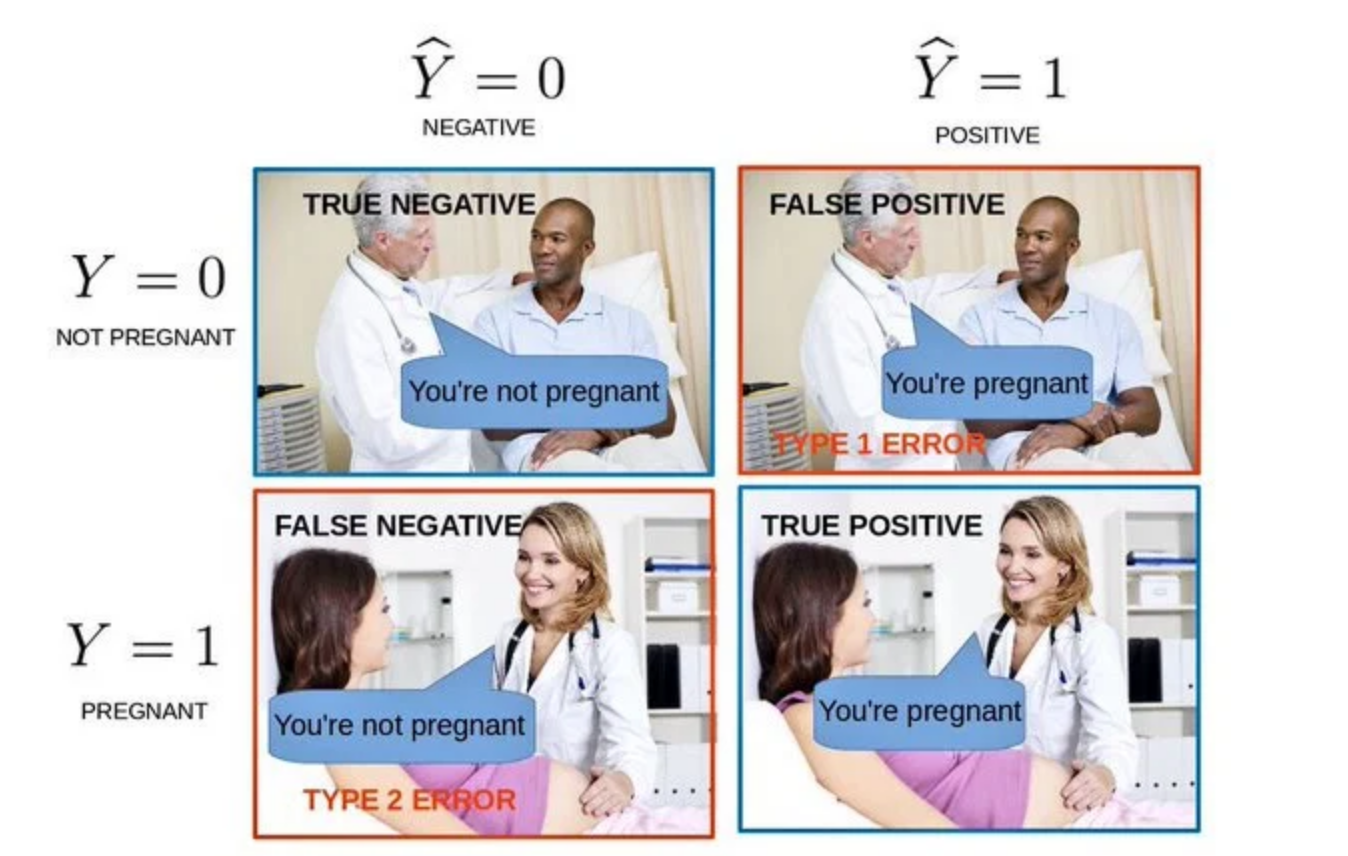
\includegraphics[scale=0.4]{../Lecture19/figures/confusion_matrix}
              \\
              \tiny
              Source: \url{https://dzone.com/articles/understanding-the-confusion-matrix}
 \end{figure}

\end{frame}


%----------------------------------------------------------------------%
\begin{frame}[fragile]
\frametitle{Probability, Cost, and Classification}

\begin{itemize}
  \item Two states of nature $y \rightarrow n\in\{0,1\}$
  \medskip
  \item Two actions $(\hat{y}) \rightarrow a\in \{0,1\}$
  \medskip
  \item Probabilities
  \begin{itemize}
    \item $p=Pr(y=1|X)$
    \item $1-p=Pr(y=0|X)$
  \end{itemize}
  \medskip
  \item Loss: $L(a,n)$, penalizes being in bin $(a,n)$
  \item Risk: expected loss of taking action $a$
\end{itemize}


\end{frame}
%----------------------------------------------------------------------%
\begin{frame}[fragile]
\frametitle{Probability, Cost, and Classification}

\begin{itemize}
  \item Risk: expected loss of taking action $a$
\end{itemize}

\begin{align}
E[L(a,n)] &= \sum_n p_n L(a,n) \\ \nonumber
R(a) &= (1-p) L(a,0) + p L(a,1)
\end{align}

\begin{itemize}
  \item The objective is the same as before: minimize the risk
  \item We have to define $L(a,n):$
  \pause
  \begin{align}
  L(n,a)=\begin{cases}
          1 & if\,\, a\neq n\\
          0 & if \,\, a=n
          \end{cases}
  \end{align}
\end{itemize}

\end{frame}
%----------------------------------------------------------------------%
\begin{frame}[fragile]
\frametitle{Probability, Cost, and Classification}

\begin{itemize}
  \item Which action do we choose?
 \bigskip
 \pause
  \item We can compare the risk of each action
  \medskip
  \item We are going to choose to take action 1 when the risk is lower:
\end{itemize}

\begin{align}
R(1) &< R(0) \\ \nonumber
1-p &< p \\ \nonumber
p &> \frac{1}{2} \\ \nonumber
\end{align}

\begin{itemize}
  \item This is known as the Bayes Classifier, choose the estate that minimizes the risk
\end{itemize}
\end{frame}

%----------------------------------------------------------------------%
\begin{frame}[fragile]
\frametitle{Probability, Cost, and Classification}

\begin{itemize}
  \item Under a 0-1 penalty the problem boils down to finding $p=Pr(y=1|X)$
  \medskip
  \item We then predict 1 if $p>0.5$ and 0 otherwise (Bayes classifier)
  \medskip
  \item We can think 4 ways of finding this probability in binary cases
  \begin{itemize}
    \item K-Nearest Neighbors
    \item Logistic
    \item Probit
    \item LDA
  \end{itemize}
\medskip
  \item But there's a trade off each time we choose a classification rule
\end{itemize}


\end{frame}
%----------------------------------------------------------------------%
\begin{frame}[fragile]
\frametitle{ROC}


\begin{columns}[T] % align columns
\begin{column}{.52\textwidth}
\begin{itemize}
\item ROC curve illustrates the trade-off of the classification rule
\medskip
\item Gives us the ability
\begin{itemize}
  \item Measure the predictive capacity of our model
  \medskip
  \item $\,$
  \medskip
\end{itemize}
\end{itemize}
\end{column}  
\hfill
\begin{column}{.48\textwidth}

 \begin{figure}[H] \centering
            \captionsetup{justification=centering}
              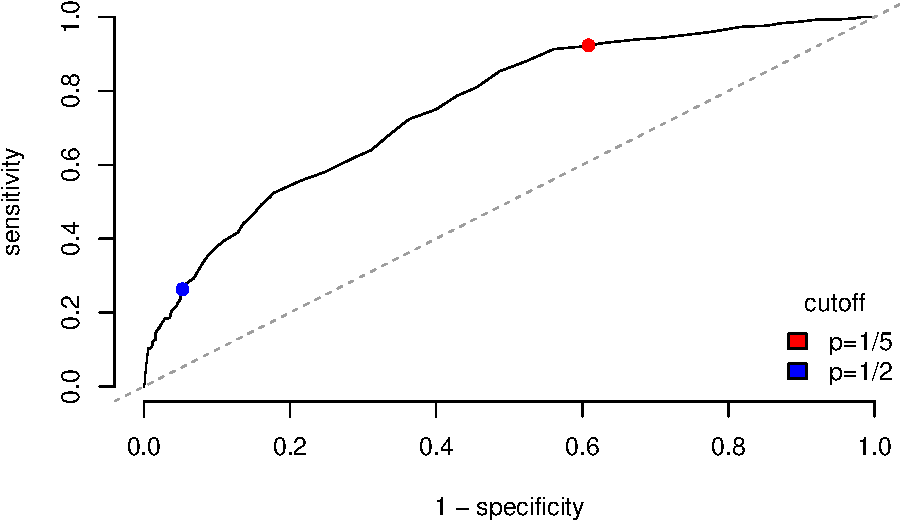
\includegraphics[scale=0.4]{../Lecture19/figures/roc}                            
 \end{figure}

\end{column}
\end{columns}


\end{frame}
%----------------------------------------------------------------------%
\begin{frame}[fragile]
\frametitle{ROC}



\begin{columns}[T] % align columns
\begin{column}{.52\textwidth}
\begin{itemize}
\item ROC curve illustrates the trade-off of the classification rule
\medskip
\item Gives us the ability
\begin{itemize}
  \item Measure the predictive capacity of our model
  \medskip
  \item Compare between models  like an $R^2$
  \medskip
\end{itemize}
\end{itemize}
\end{column}  
\hfill
\begin{column}{.48\textwidth}

 \begin{figure}[H] \centering
            \captionsetup{justification=centering}
              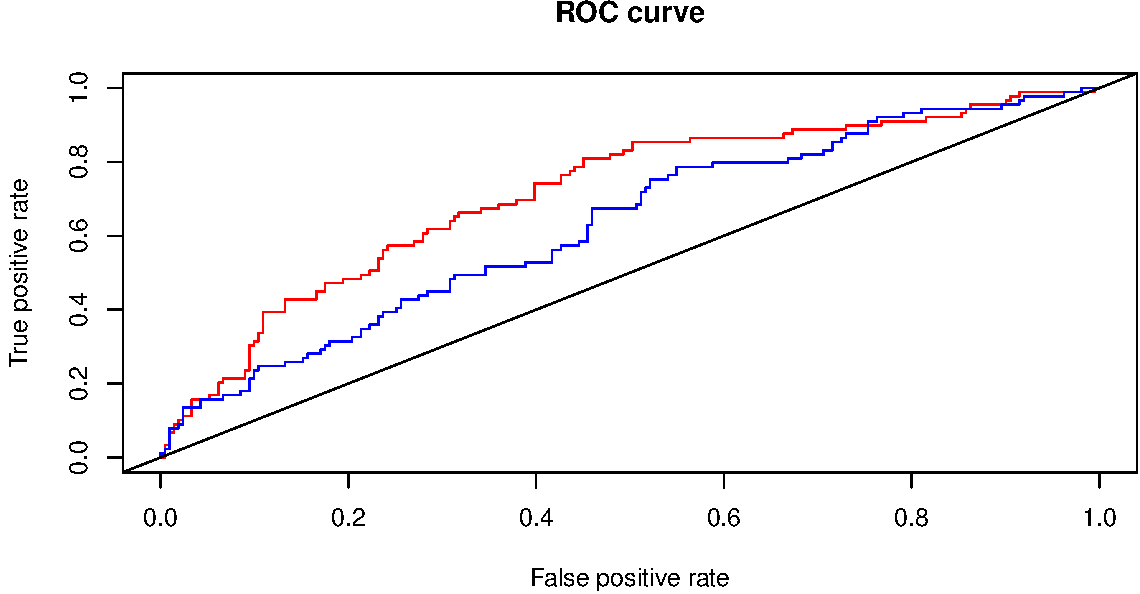
\includegraphics[scale=0.38]{../Lecture19/figures/unnamed-chunk-11-1.pdf}
 \end{figure}

\end{column}
\end{columns}



\end{frame}
%----------------------------------------------------------------------%
\begin{frame}[fragile]
\frametitle{}


\centering
{\huge \textcolor{andesred}{Trees}}



\end{frame}
%----------------------------------------------------------------------%
\section{Trees}
\subsection{Motivation}
%----------------------------------------------------------------------%
\begin{frame}[fragile]
\frametitle{Motivation}

\begin{itemize}
\item I'm going to change slightly the approach
\medskip
\item Inspired by Leo Breiman:

\medskip
{\scriptsize
{\it ``There are two cultures in the use of statistical modeling to reach conclusions from data. One assumes that the data are generated by a given stochastic data model. The other uses algorithmic models and treats the data mechanism as unknown.'' Breiman [2001b], p199.}
\medskip

{\it ``The statistical community has been committed to the almost exclusive use of data models. This commitment has led to irrelevant theory, questionable conclusions, and has kept statisticians from working on a large range of interesting current problems. Algorithmic modeling, both in theory and practice, has developed rapidly in fields outside statistics. It can be used both on large complex data sets and as a more accurate and informative alternative to data modeling on smaller data sets. If our goal as a field is to use data to solve problems, then we need to move away from exclusive dependence on data models and adopt a more diverse set of tools.'' Breiman [2001b], p199.}
}
\end{itemize}


\end{frame}

%----------------------------------------------------------------------%
\begin{frame}[fragile]
\frametitle{Motivation}


\begin{itemize}
  \item End goal is to model $y=f(x)+\epsilon$ for predictive power
  \begin{itemize}
    \item Thus far we have imposed a lot of structure to the problem
    \begin{itemize}
      \item Linear
      \item Spatial
      \item Logit
    \end{itemize}

\medskip
  \end{itemize}
  \item Regression trees, and their extension random forests are very popular and effective methods 
  \item They are very flexibly at regression functions in settings where out-of-sample predictive power is important.
\end{itemize}


\end{frame}
%----------------------------------------------------------------------%

\begin{frame}[fragile]
\frametitle{Motivation}

 \begin{figure}[H] \centering
            \captionsetup{justification=centering}
              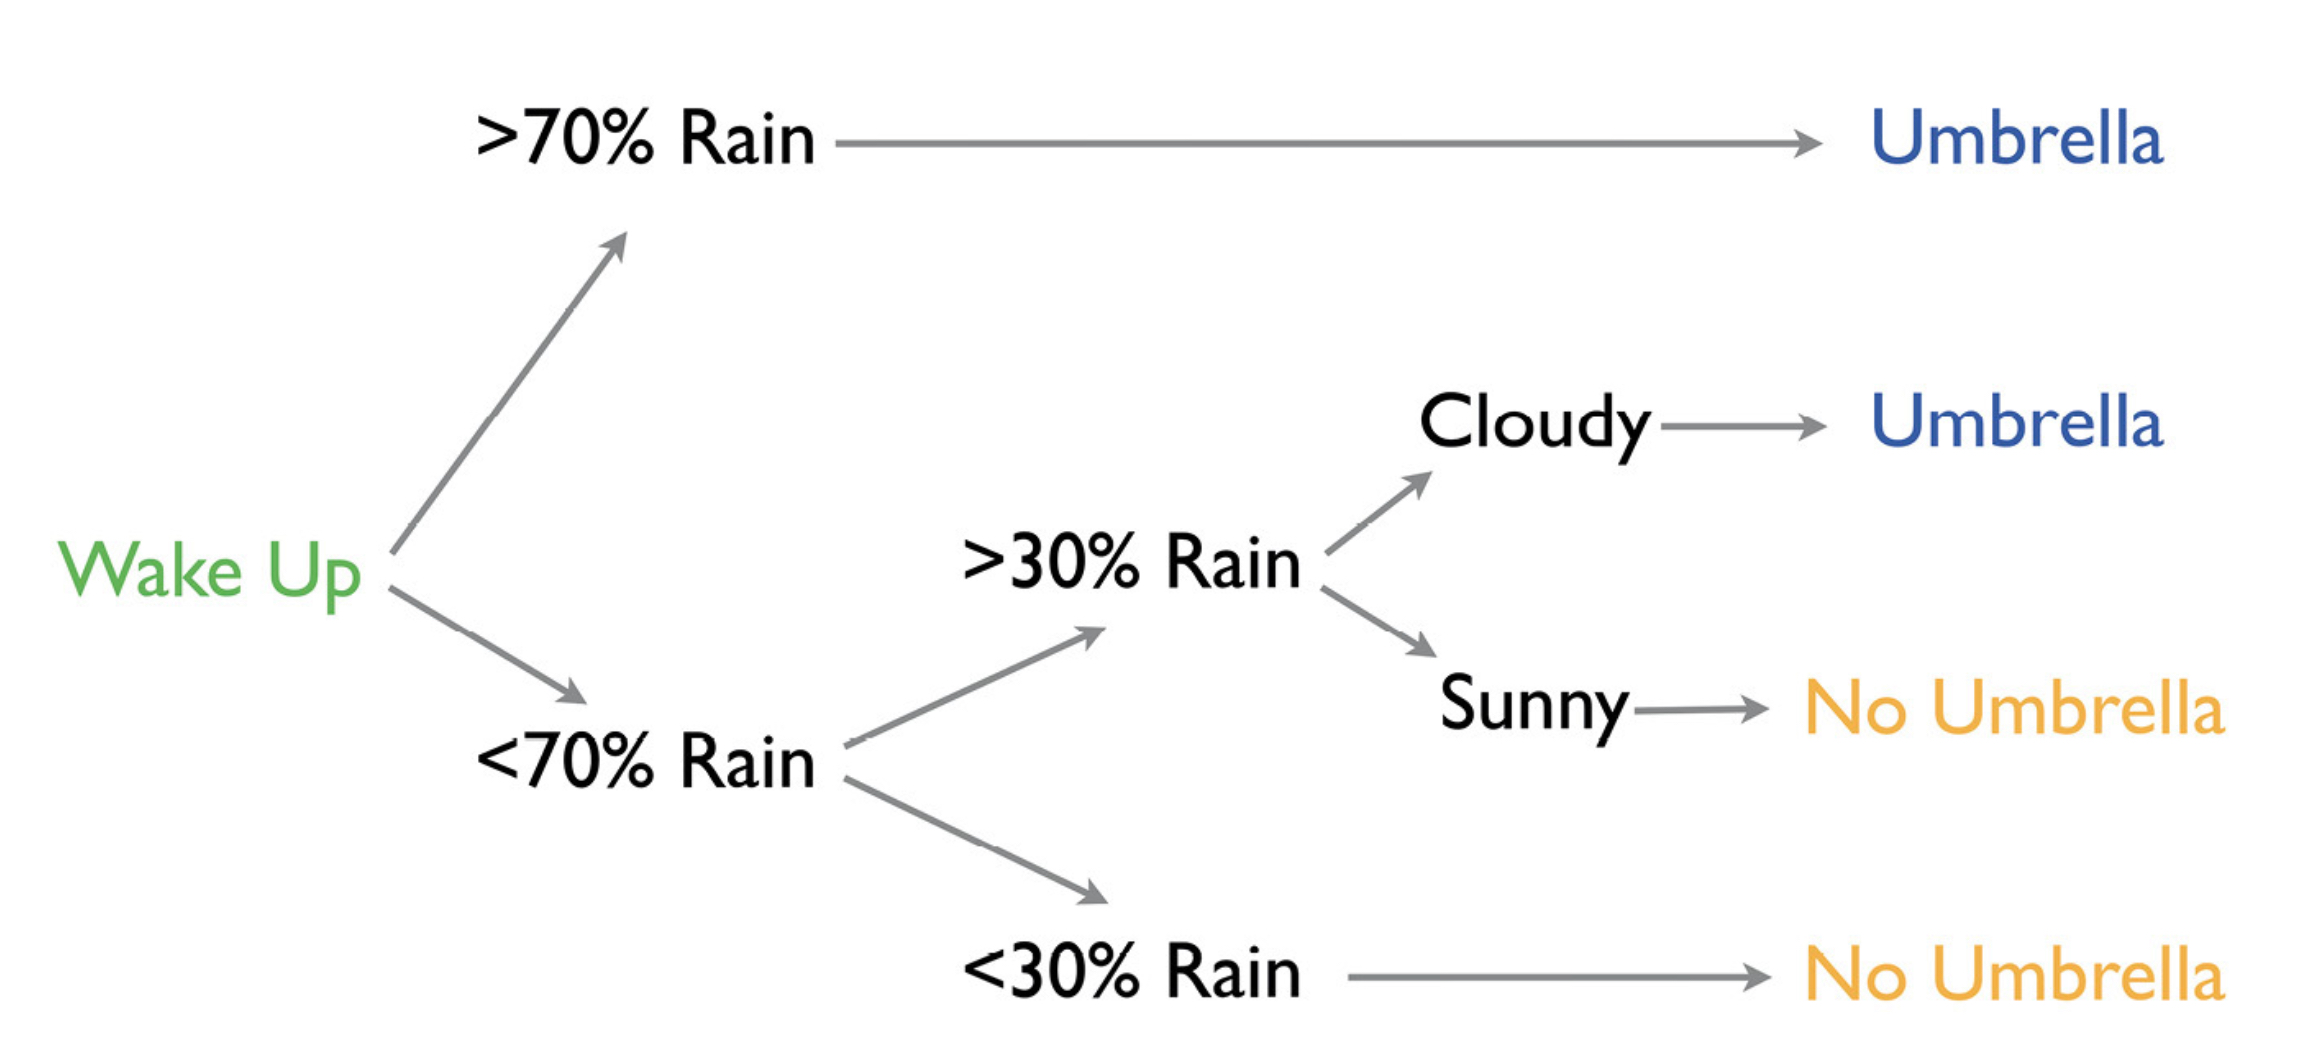
\includegraphics[scale=0.15]{figures/cart_intro}                           
 \end{figure}

\end{frame}
%----------------------------------------------------------------------%
\begin{frame}[fragile]
\frametitle{Trees: Background}


\begin{columns}[T] % align columns
\begin{column}{.42\textwidth}
  
\begin{enumerate}
\item Tree-based methods partition the feature space into a set of rectangles,
\item  fit a simple model (like a constant) in each one. 
\begin{align}
f(x) = \sum_{m=1}^M c_m I(x\in R_m)
\end{align}
\end{enumerate}


\end{column}  
\hfill
\begin{column}{.48\textwidth}

 \begin{figure}[H] \centering
            \captionsetup{justification=centering}
              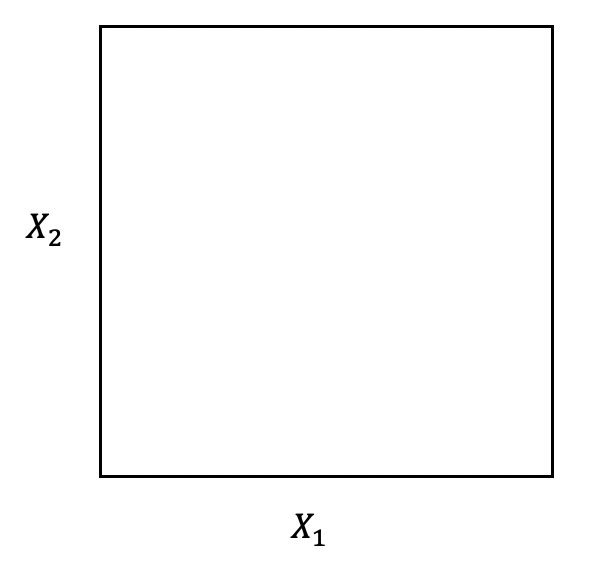
\includegraphics[scale=0.4]{figures/cart_1}                           
 \end{figure}

\end{column}
\end{columns}

\end{frame}

%----------------------------------------------------------------------%
\begin{frame}[fragile]
\frametitle{Trees: Background}


\begin{columns}[T] % align columns
\begin{column}{.42\textwidth}
  
\begin{enumerate}
\item Tree-based methods partition the feature space into a set of rectangles,
\item  fit a simple model (like a constant) in each one. 
\begin{align}
f(x) = \sum_{m=1}^M c_m I(x\in R_m)
\end{align}
\end{enumerate}


\end{column}  
\hfill
\begin{column}{.48\textwidth}

 \begin{figure}[H] \centering
            \captionsetup{justification=centering}
              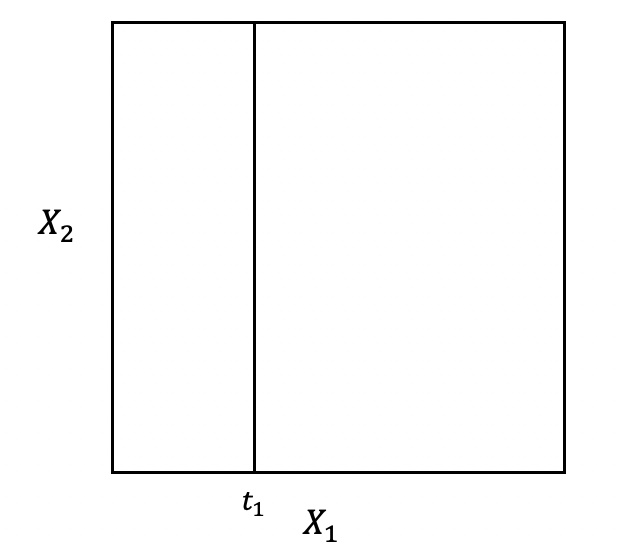
\includegraphics[scale=0.4]{figures/cart_2}                           
 \end{figure}

\end{column}
\end{columns}

\end{frame}
%----------------------------------------------------------------------%
\begin{frame}[fragile]
\frametitle{Trees: Background}


\begin{columns}[T] % align columns
\begin{column}{.42\textwidth}
  
\begin{enumerate}
\item Tree-based methods partition the feature space into a set of rectangles,
\item  fit a simple model (like a constant) in each one. 
\begin{align}
f(x) = \sum_{m=1}^M c_m I(x\in R_m)
\end{align}
\end{enumerate}


\end{column}  
\hfill
\begin{column}{.48\textwidth}

 \begin{figure}[H] \centering
            \captionsetup{justification=centering}
              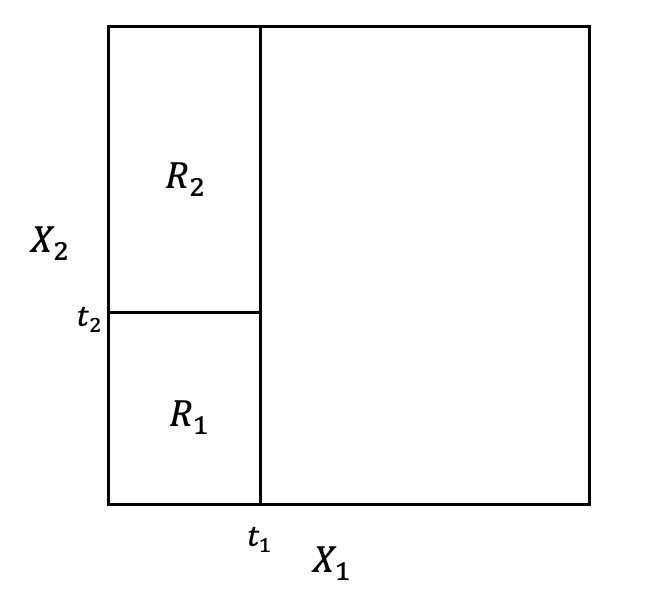
\includegraphics[scale=0.4]{figures/cart_3}                           
 \end{figure}

\end{column}
\end{columns}
\end{frame}
%----------------------------------------------------------------------%
\begin{frame}[fragile]
\frametitle{Trees: Background}


\begin{columns}[T] % align columns
\begin{column}{.42\textwidth}
  
\begin{enumerate}
\item Tree-based methods partition the feature space into a set of rectangles,
\item  fit a simple model (like a constant) in each one. 
\begin{align}
f(x) = \sum_{m=1}^M c_m I(x\in R_m)
\end{align}
\end{enumerate}


\end{column}  
\hfill
\begin{column}{.48\textwidth}

 \begin{figure}[H] \centering
            \captionsetup{justification=centering}
              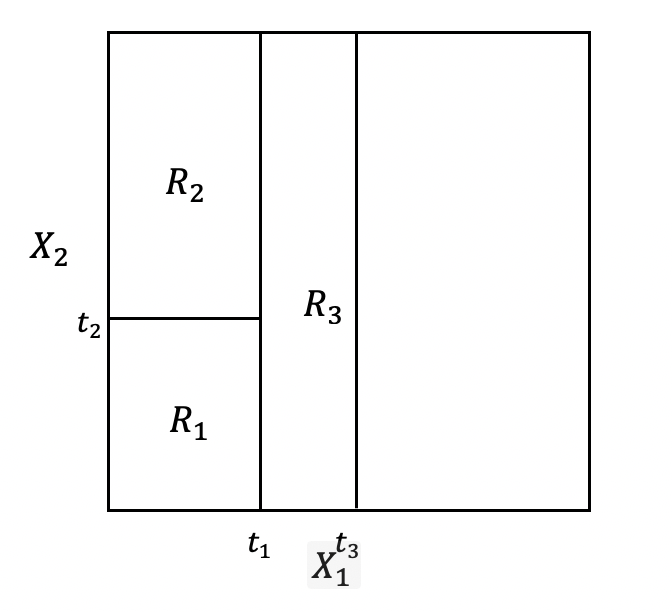
\includegraphics[scale=0.4]{figures/cart_4}                           
 \end{figure}

\end{column}
\end{columns}
\end{frame}


%----------------------------------------------------------------------%
\begin{frame}[fragile]
\frametitle{Trees: Background}


\begin{columns}[T] % align columns
\begin{column}{.42\textwidth}
  
\begin{enumerate}
\item Tree-based methods partition the feature space into a set of rectangles,
\item  fit a simple model (like a constant) in each one. 
\begin{align}
f(x) = \sum_{m=1}^M c_m I(x\in R_m)
\end{align}
\end{enumerate}


\end{column}  
\hfill
\begin{column}{.48\textwidth}

 \begin{figure}[H] \centering
            \captionsetup{justification=centering}
              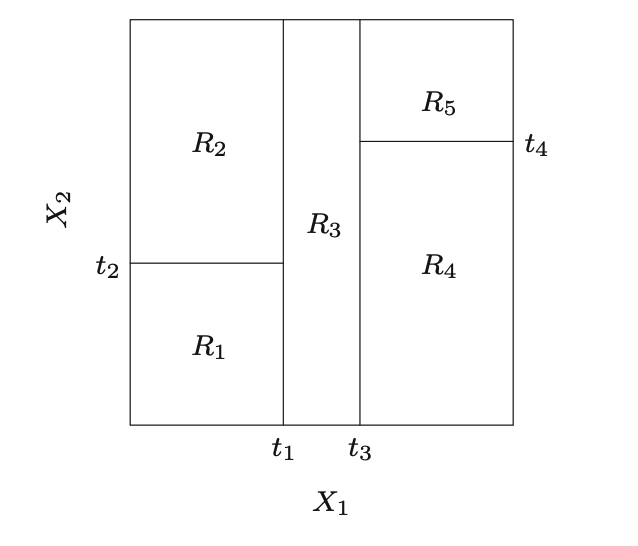
\includegraphics[scale=0.6]{figures/cart_final}                           
 \end{figure}

\end{column}
\end{columns}

\end{frame}
%----------------------------------------------------------------------%
\begin{frame}[fragile]
\frametitle{Trees: Background}


\begin{columns}[T] % align columns
\begin{column}{.42\textwidth}
  
\begin{enumerate}
\item Tree-based methods partition the feature space into a set of rectangles,
\item  fit a simple model (like a constant) in each one. 
\begin{align}
f(x) = \sum_{m=1}^M c_m I(x\in R_m)
\end{align}
\end{enumerate}


\end{column}  
\hfill
\begin{column}{.48\textwidth}

 \begin{figure}[H] \centering
            \captionsetup{justification=centering}
              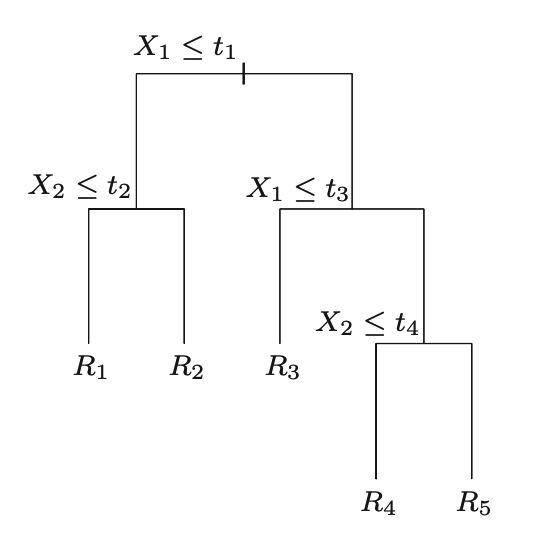
\includegraphics[scale=0.6]{figures/cart_tree}                           
 \end{figure}

\end{column}
\end{columns}


\end{frame}
%----------------------------------------------------------------------%
\begin{frame}[fragile]
\frametitle{Trees: Background}



\begin{figure}[H] \centering
            \captionsetup{justification=centering}
              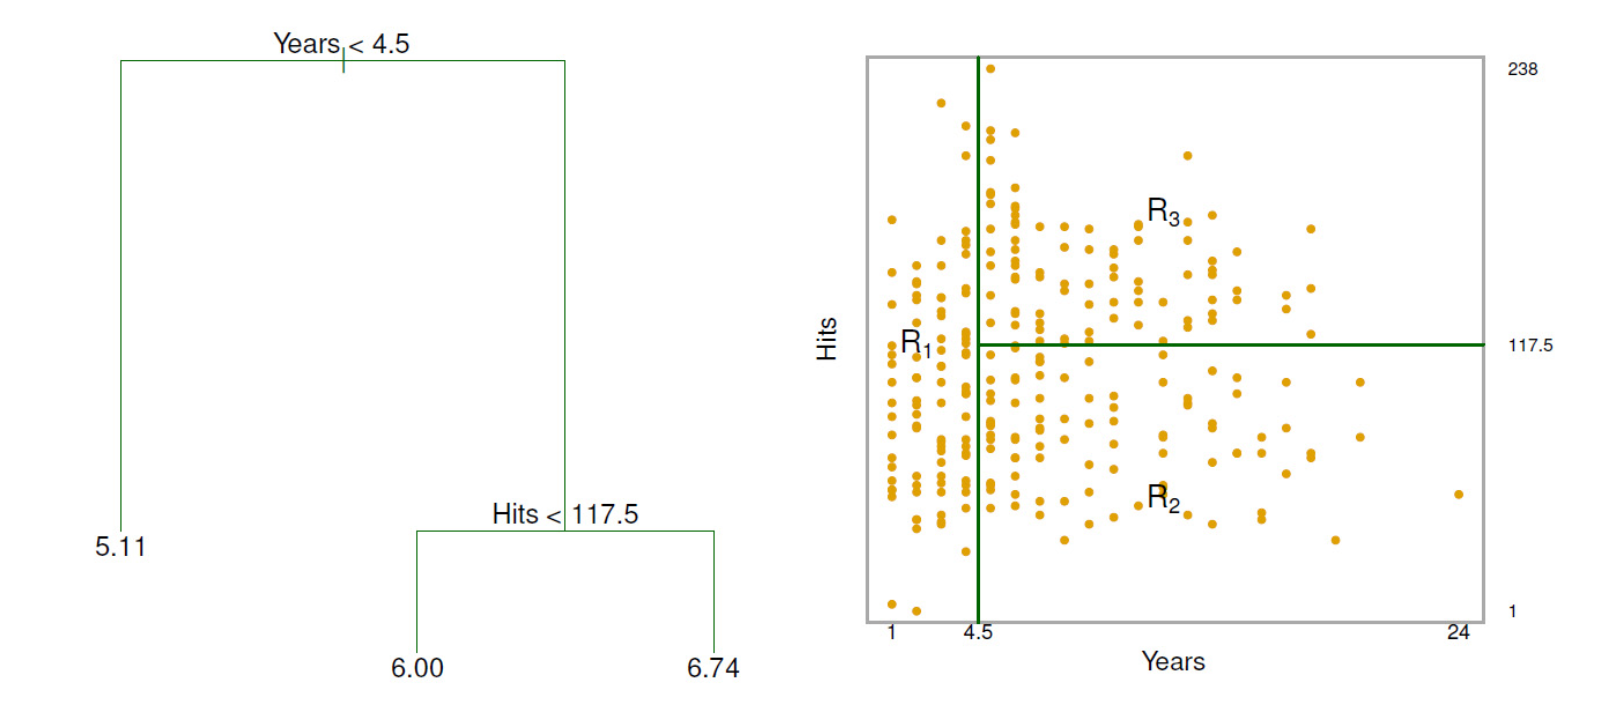
\includegraphics[scale=0.4]{figures/hitters.png}                           
 \end{figure}


\end{frame}
%----------------------------------------------------------------------%
\subsection{Regression Trees}
%----------------------------------------------------------------------%
\begin{frame}[fragile]
\frametitle{Regression Trees}

\begin{itemize}
\item We have data $y$ $n\times 1$ (outcome) and $X$ $n\times p$ (predictors)
\item Some definitions
\begin{itemize}
\item $j$ is the partition variable and $s$ is the partition point
\item Define the following half-planes
\begin{align}
R_1(j,s)=\{X|X_j\leq s\} \,\,\, \& \,\,\, R_2(j,s)=\{X|X_j>  s\}
\end{align}
\item Problem then boils down to searching the partition variable $X_j$ and the partition point $s$ such that
\begin{align}
\underset{j,s}{min} \left[ \underset{c_1}{min}\sum_{x_i\in R_1(j,s)}(y-c_1)^2+ \underset{c_2}{min}\sum_{x_i\in R_2(j,s)}(y-c_2)^2\right]
\end{align}
\end{itemize}
\end{itemize}
\end{frame}
%----------------------------------------------------------------------%
\begin{frame}<1>[label=how]
\frametitle{Regression Trees}

\begin{itemize}
\item For each partition variable, and partition point, the internal minimization is the mean of each region
\begin{align}
 \hat{c}_m =\frac{1}{n_m} \sum(y_i|x_i \in R_m)
\end{align}
\item Process is repeated inside each region. 
\pause
\item If the final tree has M regions then 
\begin{align}
\hat{f}(x) = \sum_{m=1}^M \hat{c}_m I(x \in R_m)
\end{align}

\end{itemize}

\end{frame}
%----------------------------------------------------------------------%
\begin{frame}[fragile]
\frametitle{Regression Trees}


\begin{figure}[H] \centering
            \captionsetup{justification=centering}
              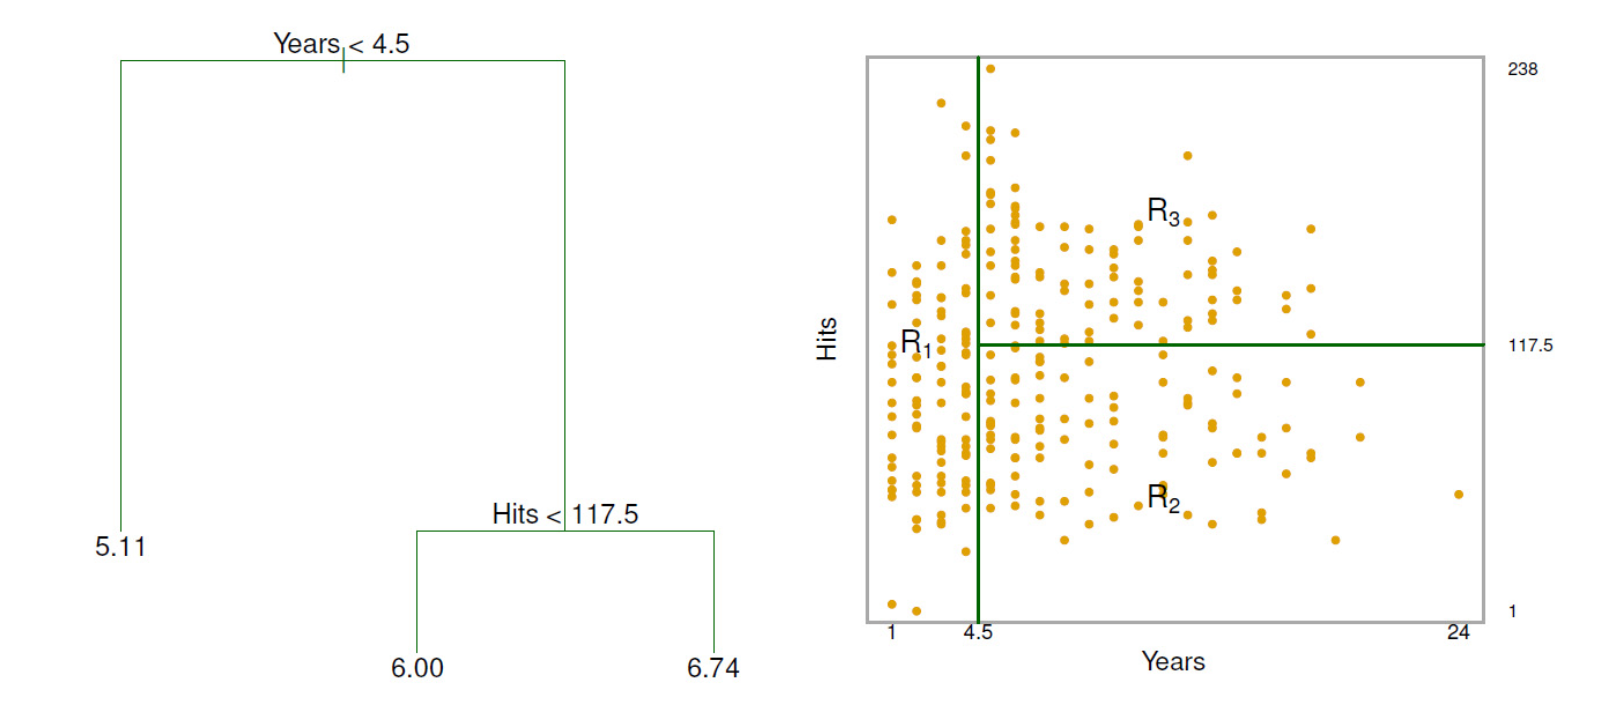
\includegraphics[scale=0.4]{figures/hitters.png}                           
 \end{figure}
\end{frame}

%----------------------------------------------------------------------%
%----------------------------------------------------------------------%
\againframe<2>{how}

%----------------------------------------------------------------------%
\begin{frame}[fragile]
\frametitle{Regression Trees}
\begin{itemize}
\item We grew our tree, now how do we stop?
\medskip
\item A tree too big, overfits the data (like a dummy for each observation)
\medskip
\item A smaller tree, with fewer splits (fewer regions $R_1,\dots,R_j$) might lead to lower variance and better interpretation at the cost of a little bias
\medskip
\item Solution: Pruning
\begin{itemize}
 \item Grow a very large tree $T_0$
 \item Prune it to get a {\it subtree}
 \item How do we determine the best way to prune the tree? $\rightarrow$ lowest test error using cross-validation
\end{itemize}

\end{itemize}

\end{frame}
%----------------------------------------------------------------------%
\begin{frame}[fragile]
\frametitle{Regression Trees}

\begin{itemize}
\item Draw back, estimate the CV error for every possible subtree would be too much (two many possible subtrees)
\medskip
\item Solution: {\it Cost complexity pruning (weakest link pruning)}
\medskip
\begin{itemize}
    \item We index the trees with $T$.
    \medskip
    \item A subtree $T \in T_0$ is a tree obtained by collapsing the terminal nodes of another tree (cutting branches).
    \medskip
    \item  $[T]$ = number of terminal nodes of tree $T$
\end{itemize}
\end{itemize}
\end{frame}
%----------------------------------------------------------------------%
\begin{frame}[fragile]
\frametitle{Regression Trees}

\begin{itemize}
\item Cost complexity of tree $T$
\begin{align}
  C_{\alpha}(T)= \sum_{m=1}^{[T]} n_m Q_m (T) + \alpha [T]
\end{align}

  \begin{itemize}
  \item where $Q_m (T)=\frac{1}{n_m} \sum_{x_i\in R_m} (y_i-\hat{c}_m)^2$ for regression trees
  \medskip
  \item  $Q_m (T)$ penalizes heterogeneity (impurity) within each region, and the second term the number of regions.
  \medskip
  \item  Objective: for a given $\alpha$, find the optimal pruning that minimizes $C_{\alpha}(T)$
  \end{itemize}
\end{itemize}
\end{frame}

%----------------------------------------------------------------------%
\begin{frame}[fragile]
\frametitle{Regression Trees}

\begin{itemize}
\item Search mechanism for $T_\alpha$ (optimal pruning given $\alpha$).
\begin{itemize}
\item Result: for each $\alpha$ there is a unique subtree $T_\alpha$ that minimizes C$\alpha$ (T).
\medskip
\item Weakest link: successively eliminate the branches that produce the minimum increase in   $\sum_{m=1}^{[T]} n_m  Q_m (T)$
\medskip
\item Idea: to remove branches is to collapse, this increases impurity, ergo, we collapse the least necessary partition.
\medskip
\item This eventually collapses at the initial node, but goes through a succession of trees, from the largest to the smallest, through the weakest link pruning process.
\medskip
\item Breiman et al. (1984): $T_\alpha$ belongs to this sequence. 
\medskip
\item Narrow your search to this succession of subtrees. 
\medskip
\item Choice of $\alpha$: cross validation.
\end{itemize}

\end{itemize}




\end{frame}
%----------------------------------------------------------------------%
\subsection{Classification Trees}
%----------------------------------------------------------------------%
\begin{frame}[fragile]
\frametitle{Classification Trees}

\begin{itemize}
\item A classification tree is very similar to a regression tree except that we try to make a prediction for a categorical rather than continuous Y.
\medskip
\item For each region (or node) we predict the most common category among the training data within that region.
\medskip
\item The tree is grown (i.e. the splits are chosen) in exactly the same way as with a regression tree except that minimizing MSE no longer makes sense.
\medskip
\item There are several possible different criteria to use %such as the “gini index” and “cross-entropy” but the easiest one to think about is to minimize the error rate.
\begin{itemize}
  \item Misclasification error: $\frac{1}{n_m}\sum_{i\in R_m} I(y_i \neq k(m))$
  \item Gini Index: $\sum_{k\neq k'}\hat{p}_{mk}\hat{p}_{mk'}=\sum_{k=1}^K \hat{p}_{mk}(1-\hat{p}_{mk})$
  \item Cross entropy or deviance: $- \sum_{k=1}^K \hat{p}_{mk}log(\hat{p}_{mk})$
\end{itemize}
\end{itemize}


\end{frame}
%----------------------------------------------------------------------%
\subsection{Advantages and disadvantages of trees}
\subsubsection{Trees vs. Linear Models}
%----------------------------------------------------------------------%
\begin{frame}[fragile]
\frametitle{Trees vs. Linear Models}
\begin{itemize}
\item Which model is better?

\begin{itemize}
  \item If the relationship between the predictors and response is linear, then classical linear models such as linear regression would outperform regression trees
  \item On the other hand, if the relationship between the predictors is non-linear, then decision trees would outperform classical approaches
\end{itemize}
\end{itemize}


\begin{columns}[T] % align columns
\begin{column}{.42\textwidth}
\scriptsize
\begin{itemize}  
\item Top row: the true decision boundary is linear
  \begin{itemize}
    \scriptsize
    \item Left: linear model (good)
    \item Right: decision tree 
  \end{itemize}

\item Bottom row: the true decision boundary is non-linear
  \begin{itemize}
    \scriptsize
    \item Left: linear model 
    \item Right: decision tree (good)
  \end{itemize}

\end{itemize}


\end{column}  
\hfill
\begin{column}{.48\textwidth}

 \begin{figure}[H] \centering
            \captionsetup{justification=centering}
              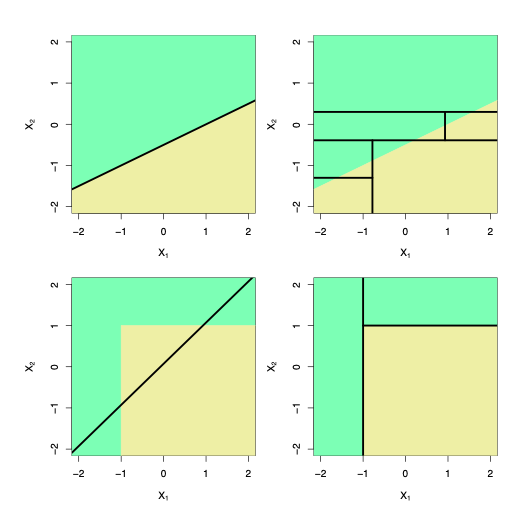
\includegraphics[scale=0.55]{figures/tree_vs_reg}
 \end{figure}

\end{column}
\end{columns}




\end{frame}
%----------------------------------------------------------------------%
\subsubsection{Advantages and disadvantages of trees}
%----------------------------------------------------------------------%
\begin{frame}[fragile]
\frametitle{Advantages and disadvantages of trees}

\begin{itemize}
\item Pros: 
  \begin{itemize}
    \item Trees are very easy to explain to people (probably even easier than linear regression)
    \medskip
    \item Trees can be plotted graphically, and are easily interpreted even by non-expert. More important variables at the top
    \medskip
    \item They work fine on both classification and regression problems
  \end{itemize}

\bigskip
\item  Cons:
  \begin{itemize}
    \item Trees are not very accurate or robust (bagging, random forests and boosting to the rescue)
    \medskip
    \item If the structure is lineal, CART doesn't work well
  \end{itemize}
\end{itemize}

\end{frame}
%----------------------------------------------------------------------%
\section{Review \& Next Steps}
%----------------------------------------------------------------------%
\begin{frame}
\frametitle{Review \& Next Steps}

\begin{itemize} 
    \item Trees
    \item Regression Trees
    \item Classification Trees
    \item  Advantages and disadvantages of trees
    \item  CART Demo

    \bigskip  
  \item  Next class:  more on trees


\bigskip  
\item Questions? Questions about software? 

\end{itemize}
\end{frame}
%----------------------------------------------------------------------%
\section{Further Readings}
%----------------------------------------------------------------------%
\begin{frame}
\frametitle{Further Readings}

\begin{itemize}
\scriptsize
  \item Athey, S., \& Imbens, G. W. (2019). Machine learning methods that economists should know about. Annual Review of Economics, 11, 685-725.
  \medskip
  \item Leo Breiman. Statistical modeling: The two cultures (with comments and a rejoinder by the author). Statistical Science, 16(3):199–231, 2001b.
  \medskip
  \item Friedman, J., Hastie, T., \& Tibshirani, R. (2001). The elements of statistical learning (Vol. 1, No. 10). New York: Springer series in statistics.
  \medskip
  \item James, G., Witten, D., Hastie, T., \& Tibshirani, R. (2013). An introduction to statistical learning (Vol. 112, p. 18). New York: springer.
  \medskip
  \item Taddy, M. (2019). Business data science: Combining machine learning and economics to optimize, automate, and accelerate business decisions. McGraw Hill Professional.
  
  
\end{itemize}

\end{frame}
%----------------------------------------------------------------------%
%----------------------------------------------------------------------%
\appendix
\newcounter{finalframe}
\setcounter{finalframe}{\value{framenumber}}
\normalsize
%----------------------------------------------------------------------%
\section{CART Demo}
\subsection{CART Demo: Regression}
%----------------------------------------------------------------------%
\begin{frame}[fragile]
\frametitle{CART Demo: Regression}

\begin{tiny}
\begin{Shaded}
\begin{Highlighting}[]
\KeywordTok{library}\NormalTok{(}\StringTok{"tree"}\NormalTok{)}

\NormalTok{prostate \textless{}{-}}\StringTok{ }\KeywordTok{read.csv}\NormalTok{(}\StringTok{"prostate.csv"}\NormalTok{)}
\KeywordTok{str}\NormalTok{(prostate)}
\end{Highlighting}
\end{Shaded}
\end{tiny}

\begin{tiny}
\begin{verbatim}
## 'data.frame':    97 obs. of  6 variables:
##  $ lcavol : num  -0.58 -0.994 -0.511 -1.204 0.751 ...
##  $ age    : int  50 58 74 58 62 50 64 58 47 63 ...
##  $ lbph   : num  -1.39 -1.39 -1.39 -1.39 -1.39 ...
##  $ lcp    : num  -1.39 -1.39 -1.39 -1.39 -1.39 ...
##  $ gleason: int  6 6 7 6 6 6 6 6 6 6 ...
##  $ lpsa   : num  -0.431 -0.163 -0.163 -0.163 0.372 ...
\end{verbatim}
\end{tiny}

\end{frame}
%----------------------------------------------------------------------%
\begin{frame}[fragile]
\frametitle{CART Demo: Regression}

\begin{scriptsize}
\begin{Shaded}
\begin{Highlighting}[]
\NormalTok{pstree \textless{}{-}}\StringTok{ }\KeywordTok{tree}\NormalTok{(lcavol }\OperatorTok{\textasciitilde{}}\NormalTok{., }\DataTypeTok{data=}\NormalTok{prostate, }\DataTypeTok{mincut=}\DecValTok{1}\NormalTok{)}
\KeywordTok{par}\NormalTok{(}\DataTypeTok{mfrow=}\KeywordTok{c}\NormalTok{(}\DecValTok{1}\NormalTok{,}\DecValTok{1}\NormalTok{))}
\KeywordTok{plot}\NormalTok{(pstree, }\DataTypeTok{col=}\DecValTok{8}\NormalTok{)}
\KeywordTok{text}\NormalTok{(pstree, }\DataTypeTok{digits=}\DecValTok{2}\NormalTok{)}
\end{Highlighting}
\end{Shaded}
\end{scriptsize}


\begin{figure}[H] \centering
            \captionsetup{justification=centering}
              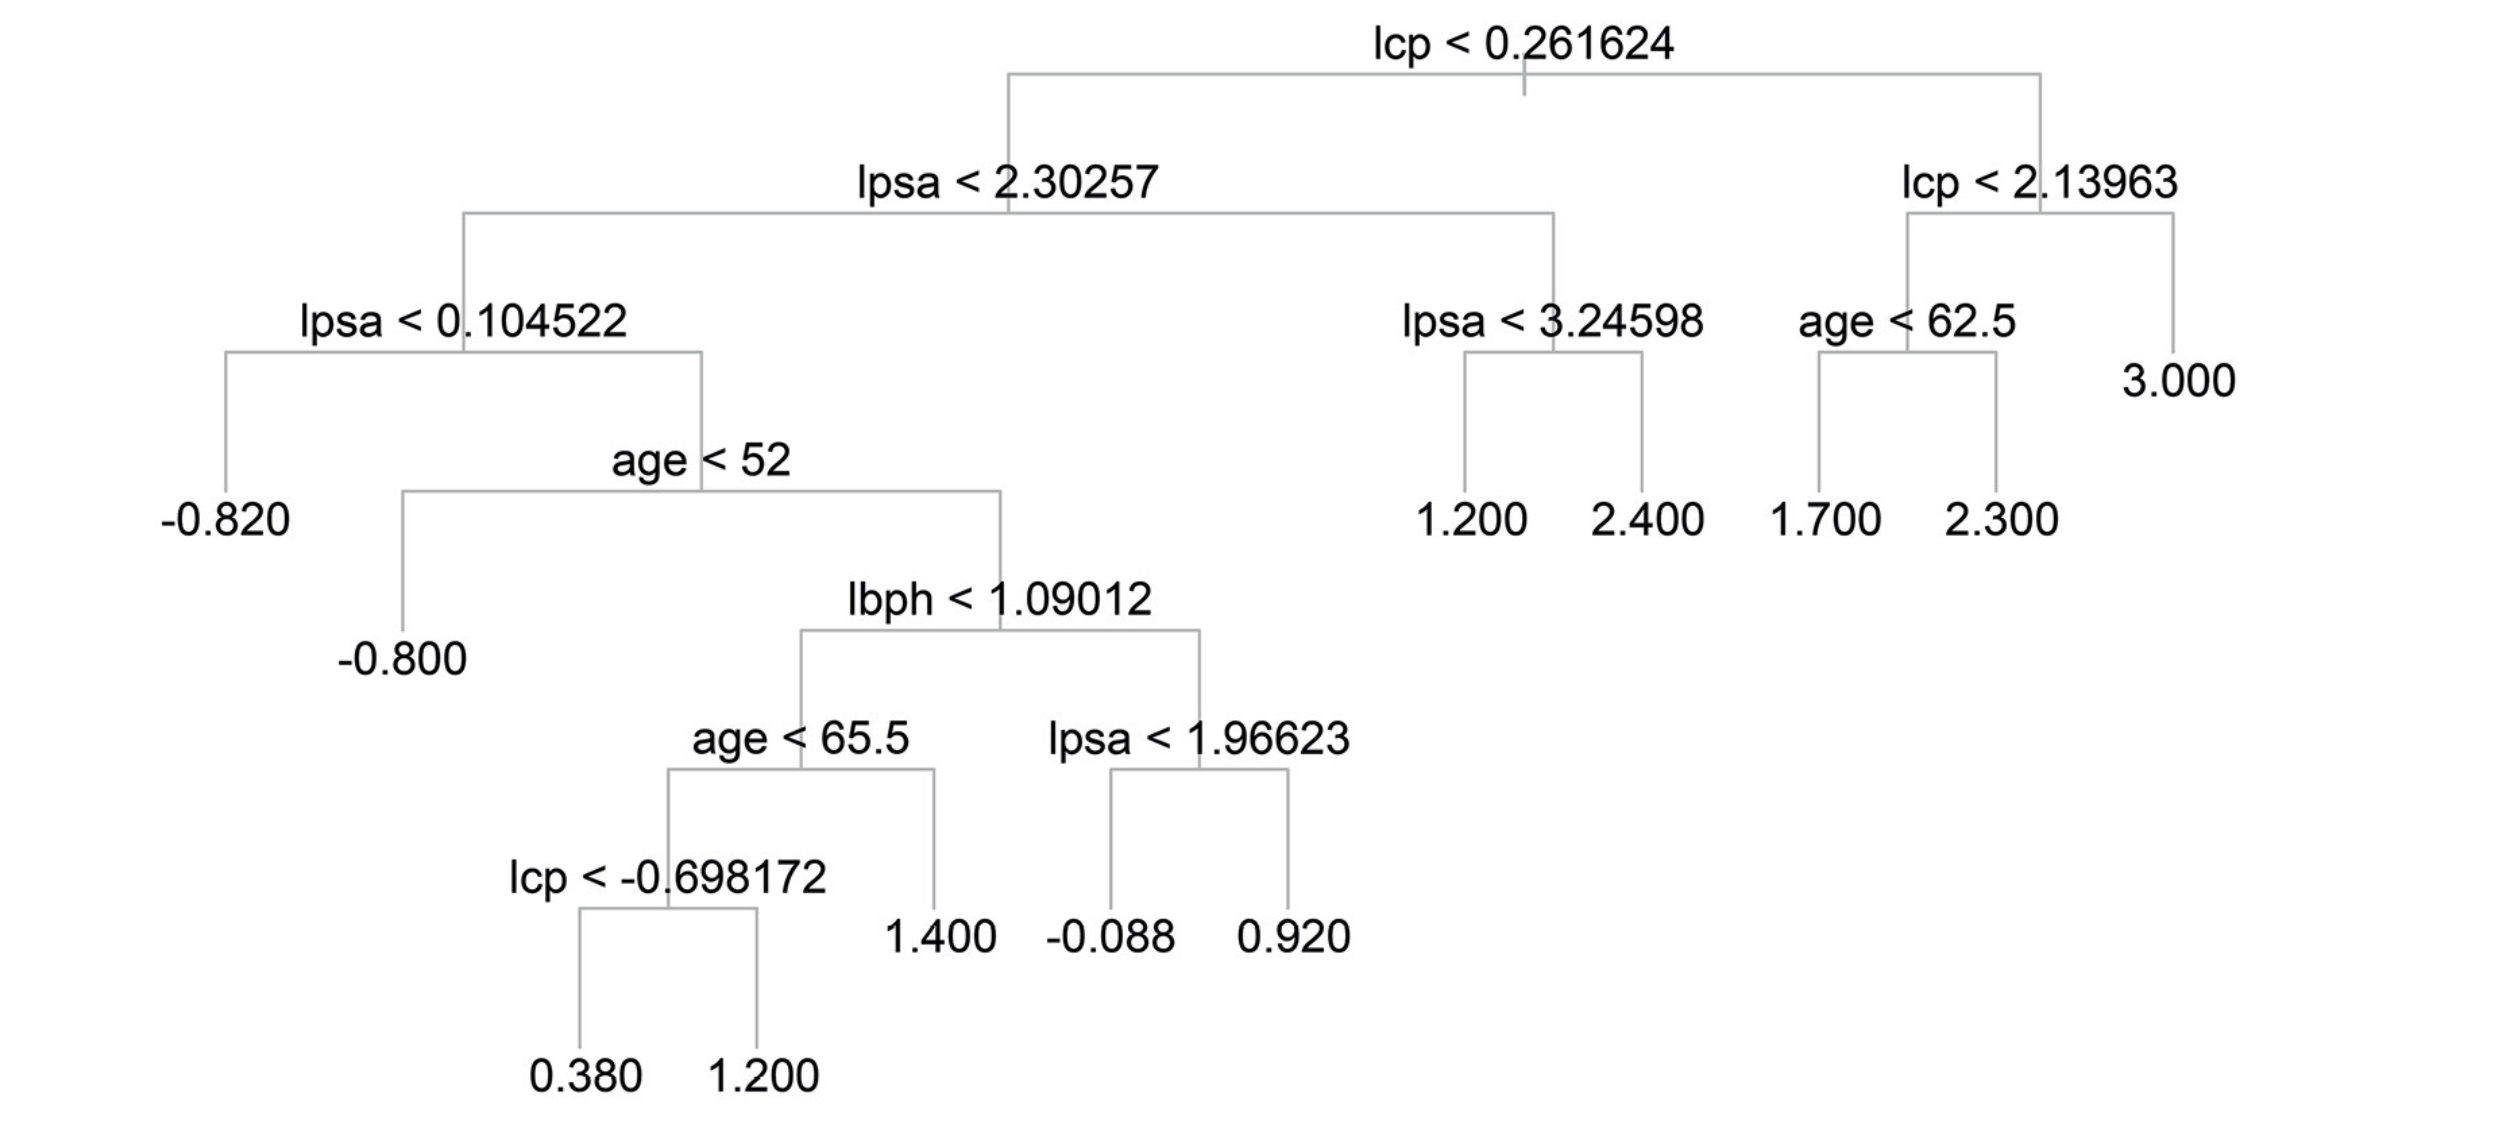
\includegraphics[scale=0.15]{figures/tree_cancer}
 \end{figure}
\end{frame}
%----------------------------------------------------------------------%
\begin{frame}[fragile]
\frametitle{CART Demo: Regression}

\begin{scriptsize}
\begin{Shaded}
\begin{Highlighting}[]
\CommentTok{\#\# Use cross{-}validation to prune the tree}
\NormalTok{cvpst \textless{}{-}}\StringTok{ }\KeywordTok{cv.tree}\NormalTok{(pstree, }\DataTypeTok{K=}\DecValTok{10}\NormalTok{)}
\KeywordTok{par}\NormalTok{(}\DataTypeTok{mai=}\KeywordTok{c}\NormalTok{(.}\DecValTok{8}\NormalTok{,.}\DecValTok{8}\NormalTok{,}\FloatTok{0.1}\NormalTok{,}\FloatTok{0.1}\NormalTok{))}
\KeywordTok{plot}\NormalTok{(cvpst}\OperatorTok{$}\NormalTok{size, cvpst}\OperatorTok{$}\NormalTok{dev, }\DataTypeTok{xlab=}\StringTok{"size"}\NormalTok{, }\DataTypeTok{ylab=}\StringTok{"oos deviance"}\NormalTok{, }\DataTypeTok{pch=}\DecValTok{21}\NormalTok{, }\DataTypeTok{bg=}\StringTok{"lightblue"}\NormalTok{, }\DataTypeTok{bty=}\StringTok{"n"}\NormalTok{)}
\end{Highlighting}
\end{Shaded}
\end{scriptsize}

\begin{figure}[H] \centering
            \captionsetup{justification=centering}
              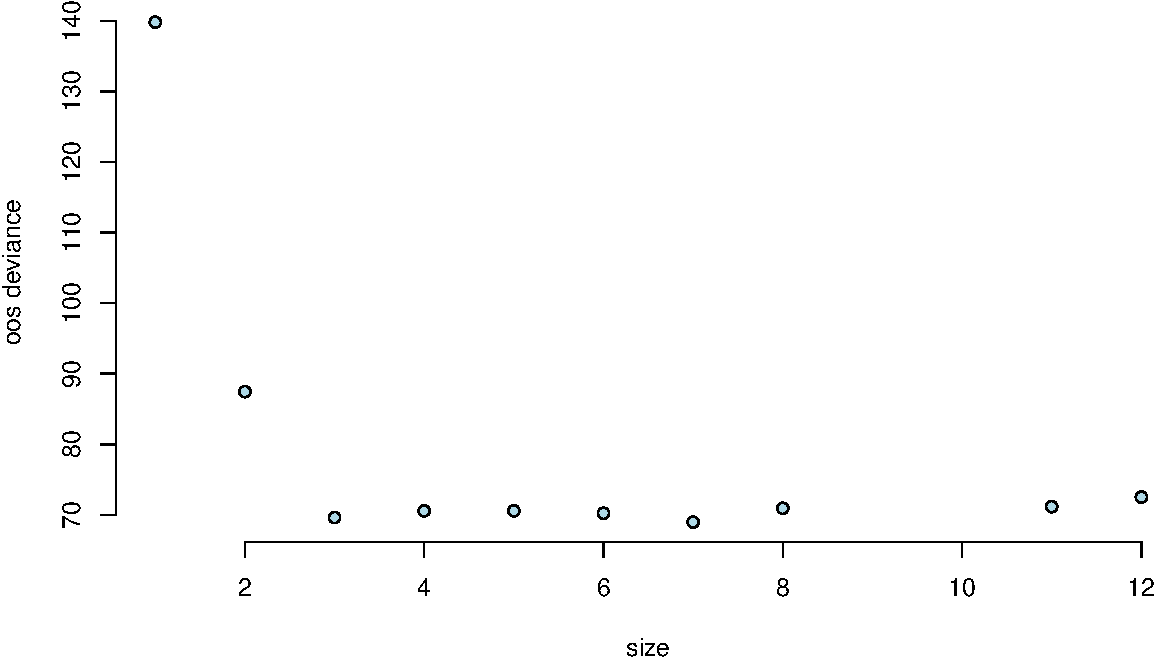
\includegraphics[scale=0.35]{figures/unnamed-chunk-4-1.pdf}
 \end{figure}


\end{frame}
%----------------------------------------------------------------------%
\begin{frame}[fragile]
\frametitle{CART Demo: Regression}

\begin{scriptsize}
\begin{Shaded}
\begin{Highlighting}[]
\KeywordTok{par}\NormalTok{(}\DataTypeTok{mfrow=}\KeywordTok{c}\NormalTok{(}\DecValTok{1}\NormalTok{,}\DecValTok{2}\NormalTok{))}
\CommentTok{\#\# note across the top is \textquotesingle{}average number of observations per leaf\textquotesingle{}; }
\KeywordTok{plot}\NormalTok{(cvpst, }\DataTypeTok{pch=}\DecValTok{21}\NormalTok{, }\DataTypeTok{bg=}\DecValTok{8}\NormalTok{, }\DataTypeTok{type=}\StringTok{"p"}\NormalTok{, }\DataTypeTok{cex=}\FloatTok{1.5}\NormalTok{, }\DataTypeTok{ylim=}\KeywordTok{c}\NormalTok{(}\DecValTok{65}\NormalTok{,}\DecValTok{100}\NormalTok{))}
\NormalTok{pstcut \textless{}{-}}\StringTok{ }\KeywordTok{prune.tree}\NormalTok{(pstree, }\DataTypeTok{best=}\DecValTok{3}\NormalTok{)}

\end{Highlighting}
\end{Shaded}
\end{scriptsize}

\begin{figure}[H] \centering
            \captionsetup{justification=centering}
              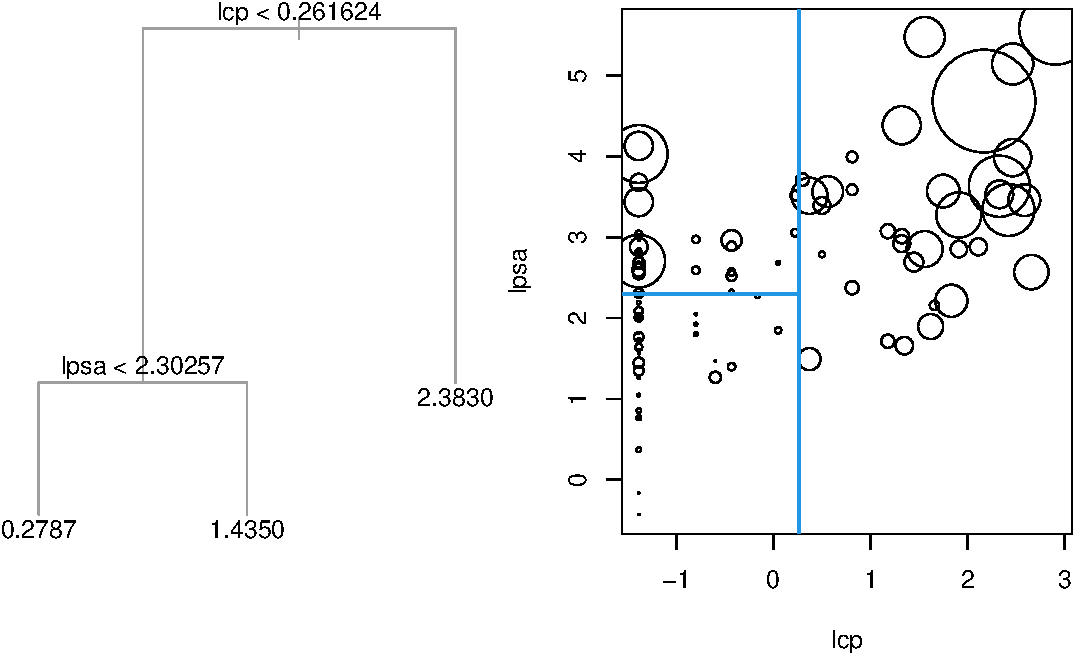
\includegraphics[scale=0.55]{figures/unnamed-chunk-6-1.pdf}
 \end{figure}


\end{frame}
%----------------------------------------------------------------------%
\subsection{CART Demo: Classification}
%----------------------------------------------------------------------%
\begin{frame}[fragile]
\frametitle{CART Demo: Classification}


\begin{scriptsize}
\begin{Shaded}
\begin{Highlighting}[]
\CommentTok{\#\# read in the NBC show characteristics}
\NormalTok{nbc \textless{}{-}}\StringTok{ }\KeywordTok{read.csv}\NormalTok{(}\StringTok{"nbc\_showdetails.csv"}\NormalTok{)}
\CommentTok{\#\# lets look at the show demographics for predicting genre}
\NormalTok{demos \textless{}{-}}\StringTok{ }\KeywordTok{read.csv}\NormalTok{(}\StringTok{"nbc\_demographics.csv"}\NormalTok{, }\DataTypeTok{row.names=}\DecValTok{1}\NormalTok{)}
\NormalTok{demos}\OperatorTok{$}\NormalTok{genre \textless{}{-}}\StringTok{ }\KeywordTok{as.factor}\NormalTok{(nbc}\OperatorTok{$}\NormalTok{Genre)}
\KeywordTok{head}\NormalTok{(demos[,}\KeywordTok{c}\NormalTok{(}\DecValTok{11}\OperatorTok{:}\DecValTok{17}\NormalTok{)])}
\end{Highlighting}
\end{Shaded}
\end{scriptsize}

\begin{tiny}
\begin{verbatim}
##                                    WIRED.CABLE.W.PAY WIRED.CABLE.W.O.PAY
## Living with Ed                               36.4929             43.6019
## Monarch Cove                                 31.2500             39.5395
## Top Chef                                     42.8806             34.1528
## Iron Chef America                            44.3794             29.9661
## Trading Spaces: All Stars                    46.4945             34.5018
## Lisa Williams: Life Among the Dead           36.7206             35.3349
##                                    DBS.OWNER BROADCAST.ONLY VIDEO.GAME.OWNER
## Living with Ed                       20.2607          0.000          66.4692
## Monarch Cove                         29.0132          0.000          54.7368
## Top Chef                             23.2329          0.041          50.5019
## Iron Chef America                    25.7776          0.000          56.9295
## Trading Spaces: All Stars            19.1882          0.000          49.4465
## Lisa Williams: Life Among the Dead   28.6374          0.000          51.7321
##                                    DVD.OWNER VCR.OWNER
## Living with Ed                       98.4597   90.4028
## Monarch Cove                         94.2105   74.1447
## Top Chef                             92.2557   78.0783
## Iron Chef America                    94.2408   83.6464
## Trading Spaces: All Stars            90.2214   81.1808
## Lisa Williams: Life Among the Dead   94.2263   84.9885
\end{verbatim}
\end{tiny}

\end{frame}
%----------------------------------------------------------------------%
\begin{frame}[fragile]
\frametitle{CART Demo: Classification}

\begin{scriptsize}
\begin{Shaded}
\begin{Highlighting}[]
\CommentTok{\#\# tree fit; it knows to fit a classification tree since genre is a factor.}
\NormalTok{genretree \textless{}{-}}\StringTok{ }\KeywordTok{tree}\NormalTok{(genre }\OperatorTok{\textasciitilde{}}\StringTok{ }\NormalTok{. , }\DataTypeTok{data=}\NormalTok{demos, }\DataTypeTok{mincut=}\DecValTok{1}\NormalTok{)}
\NormalTok{genretree}
\end{Highlighting}
\end{Shaded}
\end{scriptsize}

\begin{tiny}
\begin{verbatim}
## node), split, n, deviance, yval, (yprob)
##       * denotes terminal node
## 
##  1) root 40 75.800 Drama/Adventure ( 0.47500 0.42500 0.10000 )  
##    2) WIRED.CABLE.W.O.PAY < 28.6651 22 33.420 Drama/Adventure ( 0.72727 0.09091 0.18182 )  
##      4) VCR.OWNER < 83.749 5  6.730 Situation Comedy ( 0.00000 0.40000 0.60000 ) *
##      5) VCR.OWNER > 83.749 17  7.606 Drama/Adventure ( 0.94118 0.00000 0.05882 )  
##       10) TERRITORY.EAST.CENTRAL < 16.4555 16  0.000 Drama/Adventure ( 1.00000 0.00000 0.00000 ) *
##       11) TERRITORY.EAST.CENTRAL > 16.4555 1  0.000 Situation Comedy ( 0.00000 0.00000 1.00000 ) *
##    3) WIRED.CABLE.W.O.PAY > 28.6651 18 16.220 Reality ( 0.16667 0.83333 0.00000 )  
##      6) BLACK < 17.2017 15  0.000 Reality ( 0.00000 1.00000 0.00000 ) *
##      7) BLACK > 17.2017 3  0.000 Drama/Adventure ( 1.00000 0.00000 0.00000 ) *
\end{verbatim}
\end{tiny}
\end{frame}
%----------------------------------------------------------------------%
\begin{frame}[fragile]
\frametitle{CART Demo: Classification}

\begin{scriptsize}
\begin{Shaded}
\begin{Highlighting}[]
\CommentTok{\#\# tree plot}
\KeywordTok{plot}\NormalTok{(genretree, }\DataTypeTok{col=}\DecValTok{8}\NormalTok{, }\DataTypeTok{lwd=}\DecValTok{2}\NormalTok{)}
\CommentTok{\#\# print the predictive probabilities}
\KeywordTok{text}\NormalTok{(genretree, }\DataTypeTok{label=}\StringTok{"yprob"}\NormalTok{)}
\end{Highlighting}
\end{Shaded}
\end{scriptsize}

\begin{figure}[H] \centering
            \captionsetup{justification=centering}
              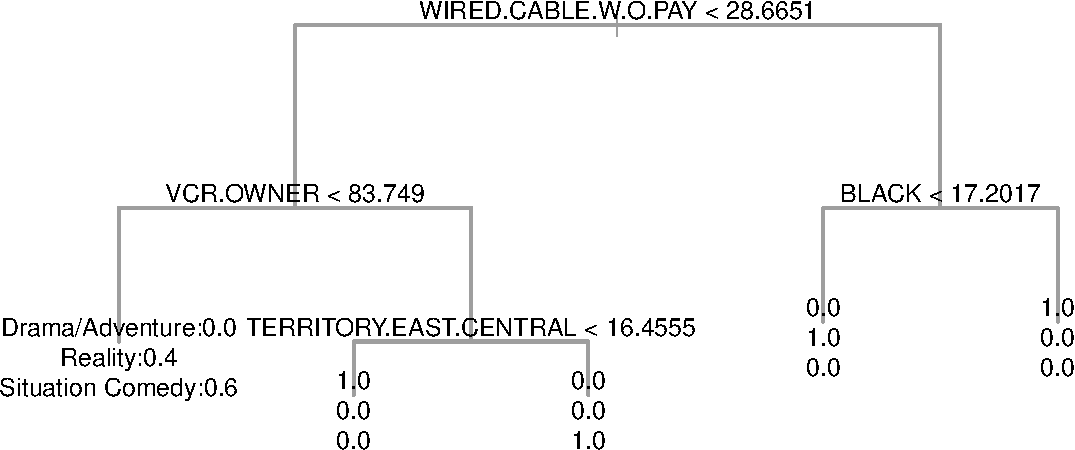
\includegraphics[scale=0.55]{figures/unnamed-chunk-9-1.pdf}
 \end{figure}



\end{frame}
%----------------------------------------------------------------------%
\begin{frame}[fragile]
\frametitle{CART Demo: Classification}

\begin{scriptsize}
\begin{Shaded}
\begin{Highlighting}[]
\CommentTok{\#\# example of prediction (type="class"  to get max prob classifications back)}
\NormalTok{genrepred \textless{}{-}}\StringTok{ }\KeywordTok{predict}\NormalTok{(genretree, }\DataTypeTok{newdata=}\NormalTok{demos, }\DataTypeTok{type=}\StringTok{"class"}\NormalTok{)}
\NormalTok{genrepred}
\end{Highlighting}
\end{Shaded}
\end{scriptsize}

\begin{tiny}
\begin{verbatim}
##  [1] Reality          Drama/Adventure  Reality          Reality         
##  [5] Reality          Reality          Reality          Reality         
##  [9] Reality          Reality          Reality          Reality         
## [13] Reality          Drama/Adventure  Drama/Adventure  Drama/Adventure 
## [17] Drama/Adventure  Drama/Adventure  Situation Comedy Drama/Adventure 
## [21] Drama/Adventure  Drama/Adventure  Situation Comedy Situation Comedy
## [25] Situation Comedy Drama/Adventure  Reality          Drama/Adventure 
## [29] Drama/Adventure  Drama/Adventure  Reality          Drama/Adventure 
## [33] Situation Comedy Drama/Adventure  Situation Comedy Drama/Adventure 
## [37] Reality          Drama/Adventure  Drama/Adventure  Drama/Adventure 
## Levels: Drama/Adventure Reality Situation Comedy
\end{verbatim}
\end{tiny}



\end{frame}

%----------------------------------------------------------------------%
%----------------------------------------------------------------------%
\end{document}
%----------------------------------------------------------------------%
%----------------------------------------------------------------------%

